\documentclass[journal,10pt,twocolumn]{IEEEtran}

\usepackage{cite}
\usepackage{graphicx}
\usepackage{amsmath,amssymb,amsfonts,amsthm}
\usepackage{algorithmic}
\usepackage{textcomp}
\usepackage{xcolor}
\usepackage{xurl}
\usepackage{microtype}
\usepackage{booktabs}
\usepackage{tabularx}
\usepackage{listings}
\usepackage{tikz}
\usepackage{array}
\usepackage{multirow}
\usepackage[hidelinks, colorlinks=true, linkcolor=blue!70!black, citecolor=green!50!black, urlcolor=blue!60!black]{hyperref}

\usetikzlibrary{arrows.meta, shapes.geometric, positioning, fit, backgrounds}

\hyphenation{op-tical net-works semi-conduc-tor to-ken-i-za-tion}

% --- Code listing style (no frame to avoid small squares) ---
\lstdefinestyle{gostyle}{
  language=Go,
  basicstyle=\footnotesize\ttfamily,
  keywordstyle=\color{blue!70!black}\bfseries,
  commentstyle=\color{green!50!black}\itshape,
  stringstyle=\color{red!60!black},
  numberstyle=\tiny\color{gray},
  breaklines=true,
  frame=none,
  tabsize=2,
  showstringspaces=false,
  captionpos=b
}
\lstdefinestyle{pythonstyle}{
  language=Python,
  basicstyle=\footnotesize\ttfamily,
  keywordstyle=\color{blue!70!black}\bfseries,
  commentstyle=\color{green!50!black}\itshape,
  stringstyle=\color{red!60!black},
  numberstyle=\tiny\color{gray},
  breaklines=true,
  frame=none,
  tabsize=2,
  showstringspaces=false,
  captionpos=b
}
\lstdefinestyle{yamlstyle}{
  language=,
  basicstyle=\footnotesize\ttfamily,
  keywordstyle=\color{blue!70!black}\bfseries,
  commentstyle=\color{green!50!black}\itshape,
  stringstyle=\color{orange!80!black},
  numberstyle=\tiny\color{gray},
  breaklines=true,
  frame=none,
  tabsize=2,
  showstringspaces=false,
  captionpos=b
}

% --- Theorem environments ---
\newtheorem{definition}{Definition}
\newtheorem{theorem}{Theorem}
\newtheorem{property}{Property}
\renewcommand{\qedsymbol}{}

% =========================================================
\begin{document}
% =========================================================

\title{Regulatory-Embedded Consensus: A Hyperledger Fabric Architecture for Institutional Real-World Asset Tokenization}

\author{Zakaria~Rahali$^{1}$ and Aya~Belkhaouad$^{2}$%
\thanks{$^{1}$Z. Rahali is a second-year engineering student in Cybersecurity and Network Infrastructures at the Moroccan School of Engineering Sciences (EMSI), Rabat, Morocco. E-mail: \href{mailto:zakaria.rahali@emsi-edu.ma}{zakaria.rahali@emsi-edu.ma}.}%
\thanks{$^{2}$A. Belkhaouad is a second-year engineering student in Cybersecurity and Network Infrastructures at the Moroccan School of Engineering Sciences (EMSI), Rabat, Morocco. E-mail: \href{mailto:aya.belkhaouad@emsi-edu.ma}{aya.belkhaouad@emsi-edu.ma}.}%
\thanks{This research forms the architectural blueprint of the ``Blockchain: Real-World Asset Tokenization Platform'' project, demonstrating the integration of traditional finance compliance mechanisms within distributed ledger technology. Manuscript submitted April 2026.}}

\markboth{IEEE Preprint --- Tokenization of Real-World Assets, April 2026}%
{Rahali and Belkhaouad: Regulatory-Embedded Consensus for Institutional RWA Tokenization}

\maketitle

% =========================================================
\begin{abstract}
% =========================================================
Traditional securities settlement currently requires $T+2$ or $T+3$ days, trapping an estimated \$10 trillion in collateral globally and generating systemic counterparty risk \cite{ref:rwa_fsb}. The tokenization of Real-World Assets (RWA) on distributed ledgers promises to resolve these inefficiencies, yet institutional adoption is constrained by a fundamental regulatory incompatibility: public blockchains cannot natively enforce Know Your Customer (KYC), Anti-Money Laundering (AML), or the Markets in Crypto-Assets (MiCA) regulation.

In this paper, we introduce the \textit{Regulatory-Embedded Consensus} (REC) model, a formally specified architecture built on Hyperledger Fabric 2.5. Unlike prior approaches that relegate regulators to passive auditor nodes, REC elevates the regulatory authority $\mathcal{R}$ to an active, endorsing participant whose cryptographic signature is a prerequisite for any state transition. We prove that REC satisfies both \textit{safety} (no non-compliant transaction can be committed) and \textit{liveness} (compliant transactions are always eventually committed) under a non-colluding adversary model.

Our Go-based Chaincode-as-a-Service (CCaaS) implementation enforces ISIN, LEI, and ISO~4217 validations on-chain and natively implements MiCA Article~68 threshold reporting. A Python FastAPI middleware orchestrates off-chain AML analysis via a Neo4j graph database, achieving pre-submission fraud screening with an overhead of 50--100\,ms per transaction. Simulation-based projections indicate sustained throughput of 1,000--1,500 TPS under the dual-endorser policy, exceeding the requirements of institutional RWA settlement by three orders of magnitude. We present a formal model, a comparative analysis against six distributed ledger paradigms, an end-to-end asset lifecycle, implementation details with code excerpts, and a STRIDE-based threat model.
\end{abstract}

\begin{IEEEkeywords}
Real-World Assets (RWA), Tokenization, Hyperledger Fabric, Decentralized Finance (DeFi), Regulatory Compliance, MiCA, Regulatory-Embedded Consensus (REC), KYC/AML, Permissioned Blockchain, Smart Contracts.
\end{IEEEkeywords}

% =========================================================
\section{Introduction}
\label{sec:intro}
% =========================================================

\IEEEPARstart{T}{raditional} financial markets are burdened by deeply entrenched structural inefficiencies. The settlement of securities and illiquid assets under the prevailing $T+2$ or $T+3$ cycle traps an estimated \$10 trillion in collateral globally, imposes bilateral counterparty credit risk, and generates operational overhead that consumes an estimated 10\% of post-trade revenue \cite{ref:rwa_fsb, ref:ecb_dlt}. The Bank for International Settlements (BIS) identifies settlement latency as one of the principal systemic vulnerabilities in modern capital markets \cite{ref:bis_tokenisation}.

The tokenization of Real-World Assets (RWA)---the process of representing ownership rights to physical or financial assets as programmable tokens on a distributed ledger---promises to fundamentally resolve these inefficiencies. By encoding asset semantics directly in smart contracts, tokenization enables atomic delivery-versus-payment (DvP), programmable fractional ownership, and automated corporate actions such as dividend distributions and covenant enforcement, all executed with deterministic, sub-second finality \cite{ref:setl2023}.

Despite these theoretical advantages, institutional adoption has largely stalled for three compounding reasons. First, public, permissionless blockchains such as Ethereum expose transaction graphs pseudonymously, creating irreconcilable conflicts with client data privacy mandates under GDPR and MiFID~II. Second, probabilistic consensus mechanisms (Proof-of-Work or Proof-of-Stake) cannot provide the settlement finality guarantee required by central counterparties (CCPs). Third, and most critically, the European Union's Markets in Crypto-Assets (MiCA) regulation \cite{ref:mica} and the FATF Recommendation~16 for virtual asset service providers \cite{ref:fatf} impose strict reporting, governance, and transaction monitoring obligations that anonymous on-chain participants are structurally incapable of fulfilling.

Existing permissioned blockchain solutions partially address these concerns. Hyperledger Fabric \cite{ref:fabric} provides channel-based privacy and pluggable endorsement policies but, in standard deployments, assigns regulators to passive auditor roles. R3 Corda \cite{ref:corda} achieves bilateral privacy through point-to-point transaction flows but lacks a global shared state, hindering systemic surveillance. DAML \cite{ref:daml} provides a high-level smart contract language with privacy primitives but does not natively embed regulatory endorsement in the consensus path.

\textbf{Contribution.} This paper makes the following contributions. First, we formalize the \textbf{Regulatory-Embedded Consensus (REC) model}, defining a tuple of actors and a strict endorsement policy that elevates the regulatory authority to an active consensus participant. Second, we prove that REC satisfies \textbf{safety} and \textbf{liveness} under a standard non-colluding adversary model. Third, we describe a \textbf{full-stack implementation} on Hyperledger Fabric 2.5, including Go CCaaS chaincode, Python FastAPI middleware with Neo4j AML analysis, and HashiCorp Vault secret management. Fourth, we present a \textbf{simulation-based performance evaluation} and a \textbf{STRIDE threat model} characterizing the security posture of the architecture.

The remainder of this paper is organized as follows. Section~\ref{sec:related} surveys related work. Section~\ref{sec:rec} formalizes the REC model. Section~\ref{sec:comparison} presents a comparative analysis. Section~\ref{sec:arch} describes the system architecture. Section~\ref{sec:usecase} traces an end-to-end asset lifecycle. Section~\ref{sec:perf} evaluates performance. Section~\ref{sec:threat} presents the threat model. Section~\ref{sec:limits} discusses limitations. Section~\ref{sec:conclusion} concludes.

% =========================================================
\section{Related Work}
\label{sec:related}
% =========================================================

\subsection{Permissioned Blockchain Platforms}

Androulaki \textit{et al.} \cite{ref:fabric} introduced Hyperledger Fabric as a modular, permissioned blockchain operating system. Its execute-order-validate (EOV) pipeline decouples transaction simulation from consensus ordering, enabling throughputs exceeding 3,000 TPS in controlled environments \cite{ref:manevich}. However, standard Fabric deployments assign regulatory entities as channel members with read access only; they do not participate in the endorsement policy, meaning compliance validation occurs off-chain at best.

R3 Corda \cite{ref:corda} was designed explicitly for financial institutions and uses a notary-based finality model with point-to-point data sharing. While Corda achieves strong bilateral privacy, its absence of a global shared ledger complicates holistic regulatory surveillance. The DAML smart contract language \cite{ref:daml} adds a privacy-preserving execution model atop distributed ledgers, but its compliance enforcement relies on off-chain legal interpretation rather than on-chain cryptographic guarantees.

The ConsenSys Quorum platform (now Hyperledger Besu) \cite{ref:quorum} provides an Ethereum-compatible permissioned environment with private transaction groups. However, it inherits Ethereum's gas-based execution model and its compliance enforcement remains programmatic rather than structurally embedded in the consensus layer.

\subsection{Regulatory Compliance on Distributed Ledgers}

Garg \textit{et al.} \cite{ref:garg2021} survey on-chain KYC approaches across Fabric, Ethereum, and Corda, concluding that no existing platform natively enforces regulator-in-the-loop transaction validation. A regulator-as-endorser design is identified as an open research direction.

Wüst and Gervais \cite{ref:wust2018} provide a formal decision framework for choosing blockchain architectures, noting that permissioned ledgers are strictly preferable for regulated financial applications due to finality guarantees, but do not address how regulators can be embedded in the consensus protocol itself.

The European Central Bank's DLT pilot \cite{ref:ecb_dlt} experimented with central bank money settlement on permissioned ledgers and found that regulator participation as a passive observer was insufficient for real-time systemic risk monitoring, motivating the need for active regulator integration.

\subsection{RWA Tokenization Platforms}

The FSB \cite{ref:rwa_fsb} identifies the primary barriers to institutional RWA tokenization as follows: the lack of standardized on-chain legal representations, the inability to enforce AML/KYC natively, and interoperability gaps between tokenized and traditional settlement infrastructure. The BIS \cite{ref:bis_tokenisation} further notes that private ledgers with embedded regulatory logic represent the most viable near-term path for institutional adoption.

Setl \textit{et al.} \cite{ref:setl2023} implement a Fabric-based tokenization platform for equities but rely on an off-chain compliance engine. Their reported latency of 150--200\,ms per transaction demonstrates the feasibility of permissioned ledgers for institutional use but does not address the oracle dependency problem created by off-chain AML systems.

\subsection{Gap Analysis}

Across the literature surveyed, no prior work formalizes a consensus model in which a regulatory authority holds an active cryptographic endorsement role as a structural invariant of the protocol. Prior approaches either assign regulators to passive observer roles, perform compliance validation off-chain without on-chain enforcement, or rely on programmatic smart contract logic that can be bypassed by consortium administrators with sufficient access. REC addresses all three gaps by making regulatory endorsement a protocol-level prerequisite for state commitment.

% =========================================================
\section{The Regulatory-Embedded Consensus (REC) Model}
\label{sec:rec}
% =========================================================

In public blockchains, the consensus mechanism solely verifies cryptographic signatures and prevents double-spending. In our architecture, consensus is expanded to inherently guarantee deterministic regulatory compliance before any state transition is committed.

\subsection{Actor Model}

\begin{definition}[REC Actors]
The REC network $\mathcal{N}$ is defined by a tuple $\mathcal{N} = \langle \mathcal{F}, \mathcal{R}, \mathcal{O} \rangle$ where $\mathcal{F}$ is the set of \textbf{Financial Operators} (e.g., commercial banks), each operating one or more endorsing peer nodes, responsible for asset origination, client onboarding, and transaction proposal submission; $\mathcal{R}$ is the set of \textbf{Regulatory Bodies} (e.g., the AMF), each operating an independent endorsing peer node, executing compliance validation functions; and $\mathcal{O}$ is the \textbf{Ordering Service}, an EtcdRaft cluster responsible for deterministic transaction sequencing and crash fault-tolerant (CFT) finality.
\end{definition}

\subsection{Formal Endorsement Policy}

Let $\mathcal{T}$ be a proposed transaction (e.g., \texttt{TransferAsset}). Let $V_{state}(\mathcal{T})$ denote the standard world-state validity function and $V_{comp}(\mathcal{T})$ denote a compliance validation function executed exclusively by $\mathcal{R}$, evaluating KYC status, AML flags, sanction list membership, and MiCA threshold constraints.

\begin{definition}[REC Endorsement Policy]
\label{def:rec}
The REC endorsement policy $\mathbb{E}$ holds that a transaction $\mathcal{T}$ reaches committed state if and only if it carries valid cryptographic signatures from both $\mathcal{F}$ and $\mathcal{R}$:
\begin{equation*}
\label{eq:endorsement}
\mathbb{E}(\mathcal{T}) = \textit{Sign}(\mathcal{F},\, V_{state}(\mathcal{T})) \;\wedge\; \textit{Sign}(\mathcal{R},\, V_{comp}(\mathcal{T}))
\end{equation*}
\end{definition}

This shifts regulatory oversight from a reactive, post-facto audit process into a proactive, cryptographic necessity embedded in the consensus critical path.

\subsection{MiCA Threshold Event}

For any transfer of value, a secondary compliance function emits a regulatory alert when the transferred amount $v$ exceeds the MiCA Article~68 reporting threshold $\theta_{\text{MiCA}} = 1{,}000{,}000$ EUR:
\[
E_{\text{MiCA}}(\mathcal{T}) =
\left\{
\begin{aligned}
&\text{\ttfamily\footnotesize MiCAThresholdExceeded}(\\
&\quad \mathcal{T}.\mathrm{id},\, v), && \text{if } v > \theta_{\text{MiCA}}, \\
&\varnothing, && \text{otherwise.}
\end{aligned}
\right.
\]

This event is emitted atomically within the chaincode execution context and is persisted in the ledger, ensuring an immutable audit trail of all reportable transactions.

\subsection{Safety and Liveness Properties}

\begin{property}[Safety]
\label{prop:safety}
Under REC, no non-compliant transaction $\mathcal{T}$ such that $V_{comp}(\mathcal{T}) = \bot$ can reach committed state.
\end{property}

\begin{proof}[Proof Sketch]
By Definition~\ref{def:rec}, commitment requires $\textit{Sign}(\mathcal{R}, V_{comp}(\mathcal{T}))$. Since $\mathcal{R}$ only produces this signature when $V_{comp}(\mathcal{T}) = \top$, a transaction where $V_{comp}(\mathcal{T}) = \bot$ cannot satisfy $\mathbb{E}(\mathcal{T})$. The Fabric orderer rejects any transaction proposal that does not carry a complete, valid endorsement set \cite{ref:fabric}. Therefore, no non-compliant transaction can be ordered or committed.
\end{proof}

\begin{property}[Liveness]
\label{prop:liveness}
Under REC, any compliant transaction $\mathcal{T}$ such that $V_{comp}(\mathcal{T}) = \top$ and $V_{state}(\mathcal{T}) = \top$ will eventually be committed, provided $\mathcal{F}$ and $\mathcal{R}$ are both online and non-faulty.
\end{property}

\begin{proof}[Proof Sketch]
If $\mathcal{F}$ and $\mathcal{R}$ are online, both signatures in $\mathbb{E}(\mathcal{T})$ can be produced. The EtcdRaft ordering service provides CFT liveness: it makes progress as long as a majority of orderer nodes are available \cite{ref:raft}. Therefore, a fully endorsed compliant transaction will eventually be ordered and committed.
\end{proof}

\begin{theorem}[REC Safety under Non-Colluding Adversary]
\label{thm:safety}
Let adversary $\mathcal{A}$ control at most one of $\{\mathcal{F}, \mathcal{R}\}$ and any strict minority of orderer nodes. Under these conditions, $\mathcal{A}$ cannot cause any non-compliant transaction to be committed.
\end{theorem}

\begin{proof}[Proof Sketch]
Compromising $\mathcal{F}$ alone is insufficient: the endorsement policy requires $\mathcal{R}$'s signature, which $\mathcal{A}$ does not control. Compromising $\mathcal{R}$ alone is insufficient: the orderer will reject a transaction that carries only $\mathcal{R}$'s signature without $\mathcal{F}$'s. Compromising a minority of orderer nodes does not affect safety under EtcdRaft \cite{ref:raft}: the committed log cannot be altered without controlling a majority. Hence, $\mathcal{A}$ cannot forge a committed non-compliant transaction under the stated adversary model.
\end{proof}

% =========================================================
\section{Comparative Analysis}
\label{sec:comparison}
% =========================================================

Table~\ref{tab:comparison} compares the REC architecture against six distributed ledger paradigms across five dimensions relevant to institutional RWA tokenization. Ethereum's public nature precludes client data privacy and deterministic finality. Hyperledger Besu (Quorum) provides permissioned Ethereum but inherits its gas model and lacks native regulatory endorsement. R3 Corda offers bilateral privacy but no global shared state, complicating systemic surveillance. DAML provides contractual privacy primitives but relies on off-chain legal compliance. Standard Fabric allows programmable compliance but relegates regulators to passive observers. Only the REC model embeds regulatory authority as an active, cryptographically enforced consensus participant.

\begin{table*}[t]
\centering
\caption{Comparative Analysis of Distributed Ledger Paradigms for Institutional RWA Tokenization}
\label{tab:comparison}
\begin{tabularx}{\textwidth}{@{}lXXXXXX@{}}
\toprule
\textbf{Metric} & \textbf{Ethereum} & \textbf{Besu/Quorum} & \textbf{Std. Fabric} & \textbf{R3 Corda} & \textbf{DAML} & \textbf{REC (Ours)} \\
\midrule
Privacy & Pseudonymous & Private groups & Channel-based & Point-to-point & Need-to-know & Channel + reg. visibility \\
Compliance & Off-chain & Off-chain & Programmable & Notarized & Off-chain legal & \textbf{Cryptographic, pre-commit} \\
Finality & Probabilistic & Deterministic & Deterministic & Deterministic & Deterministic & Deterministic (EtcdRaft) \\
Performance & Volatile & Predictable & High & Moderate & Platform-dep. & \textbf{High, predictable} \\
Reg. integration & Impossible & Passive observer & Passive auditor & Passive observer & Passive observer & \textbf{Active endorsing peer} \\
\bottomrule
\end{tabularx}
\end{table*}

% =========================================================
\section{System Architecture}
\label{sec:arch}
% =========================================================

The REC platform is a full-stack, enterprise-grade distributed system organized in three distinct layers, as illustrated in Fig.~\ref{fig:arch}.

\begin{figure}[htbp]
\centering

\includegraphics[width=\columnwidth]{figs/fig1.png}
\caption{REC three-layer system architecture. Flow: (1)~client submits proposal via REST; (2)~middleware performs AML screening; (3)~chaincode executes on Peer~$\mathcal{F}$; (4)~Peer~$\mathcal{R}$ performs compliance endorsement; (5)~orderer sequences and broadcasts; (6)~all peers commit.}
\label{fig:arch}
\end{figure}

\subsection{Layer 1: Chaincode-as-a-Service (CCaaS)}

The core business logic is encapsulated in a Go-based smart contract deployed under the CCaaS paradigm \cite{ref:fabric}. Decoupling the chaincode process from the Fabric peer node allows independent versioning, containerized deployment, and hot-reloading of compliance logic without peer downtime.

Listing~\ref{lst:go} shows the \texttt{TransferAsset} function, illustrating on-chain ISIN validation and MiCA threshold detection.

\begin{lstlisting}[style=gostyle, caption={Go chaincode: \texttt{TransferAsset} with ISIN validation and MiCA threshold detection.}, label={lst:go}]
func (s *SmartContract) TransferAsset(
    ctx contractapi.TransactionContextInterface,
    assetID, newOwnerLEI string, amount float64,
) error {
    asset, err := s.ReadAsset(ctx, assetID)
    if err != nil { return err }
    if asset.Status == "FROZEN" {
        return fmt.Errorf("asset %s is frozen", assetID)
    }
    if len(asset.ISIN) != 12 {
        return fmt.Errorf("invalid ISIN: must be 12 chars")
    }
    if len(newOwnerLEI) != 20 {
        return fmt.Errorf("invalid LEI: must be 20 chars")
    }
    if amount > MiCAThreshold {
        ctx.GetStub().SetEvent("MiCAThresholdExceeded",
            []byte(fmt.Sprintf(
                `{"assetID":"%s","amount":%.2f}`,
                assetID, amount)))
    }
    asset.Owner = newOwnerLEI
    assetJSON, _ := json.Marshal(asset)
    return ctx.GetStub().PutState(assetID, assetJSON)
}
\end{lstlisting}

The chaincode enforces the following invariants on all state transitions. \textbf{ISIN validation} requires a 12-character alphanumeric string conforming to ISO 6166. \textbf{LEI validation} requires a 20-character string conforming to ISO 17442. \textbf{Currency validation} requires a 3-character code conforming to ISO 4217. \textbf{MiCA threshold} detection ensures that any transfer $v > 1{,}000{,}000$ EUR emits \texttt{MiCAThresholdExceeded} according to the MiCA event rule. Finally, an \textbf{asset state machine} enforces valid transitions through functions \texttt{TokenizeAsset}, \texttt{TransferAsset}, \texttt{FreezeAsset}, and \texttt{UnfreezeAsset}, as per Fig.~\ref{fig:statemachine}.

\subsection{Layer 2: High-Performance Middleware}

A Python FastAPI backend orchestrates off-chain concerns. Listing~\ref{lst:python} shows the transfer endpoint, which gates Fabric submission behind a Neo4j AML check.

\begin{lstlisting}[style=pythonstyle, caption={Python FastAPI middleware: AML pre-check before Fabric submission.}, label={lst:python}]
@router.post("/assets/{asset_id}/transfer")
async def transfer_asset(
    asset_id: str,
    req: TransferRequest,
    fabric: FabricGateway = Depends(get_fabric),
    neo4j: Neo4jDriver = Depends(get_graph),
):
    # 1. AML graph analysis (Neo4j Cypher query)
    risk = await neo4j.check_entity_risk(
        req.new_owner_lei)
    if risk.score > AML_THRESHOLD:
        raise HTTPException(403,
            "AML risk threshold exceeded")
    # 2. Submit to Fabric (triggers dual endorsement)
    tx_id = await fabric.submit_transaction(
        "TransferAsset",
        asset_id, req.new_owner_lei, str(req.amount)
    )
    return {"tx_id": tx_id, "status": "committed"}
\end{lstlisting}

The Neo4j graph database represents entities (banks, corporates, individuals) as nodes and historical transactions as directed edges. AML analysis traverses this graph using Cypher queries to detect circular fund flows, layering patterns, and connections to flagged entities---patterns that are computationally prohibitive to encode in chaincode. Secret management is delegated to HashiCorp Vault in \texttt{AppRole} mode, storing Fabric SDK credentials, API keys, and the middleware's TLS certificates with automatic rotation. Off-chain KYC documents and PII are persisted in a PostgreSQL database encrypted at rest, ensuring GDPR Article~25 data minimization compliance.

\subsection{Layer 3: Client Interface}

A React/Vite Single Page Application (SPA) provides institutional operators with a professional dashboard featuring real-time asset registry views, transaction submission forms with client-side ISIN/LEI validation, and a compliance event feed for monitoring \texttt{MiCAThresholdExceeded} alerts.

\subsection{Deployment: CCaaS with Regulatory Peer}

Listing~\ref{lst:yaml} shows the Docker Compose excerpt defining the regulatory peer as an independent Fabric organization.

\begin{lstlisting}[style=yamlstyle, caption={Docker Compose: regulatory peer as a separate Fabric organization.}, label={lst:yaml}]
services:
  peer0.regulator.example.com:
    image: hyperledger/fabric-peer:2.5
    environment:
      - CORE_PEER_ID=peer0.regulator.example.com
      - CORE_PEER_LOCALMSPID=RegulatorMSP
      - CORE_PEER_MSPCONFIGPATH=
          /etc/hyperledger/fabric/msp
      - CORE_PEER_TLS_ENABLED=true
    volumes:
      - ./crypto-config/regulatorOrg:/etc/hyperledger
    networks: [fabric_net]

  ccaas.rwa:
    image: rwa-chaincode:latest
    environment:
      - CHAINCODE_SERVER_ADDRESS=0.0.0.0:9999
      - CORE_CHAINCODE_ID_NAME=rwa:1.0
    networks: [fabric_net]
\end{lstlisting}

% =========================================================
\section{End-to-End Asset Lifecycle}
\label{sec:usecase}
% =========================================================

To illustrate REC's operational capability, we trace the lifecycle of a tokenized corporate bond, as depicted in the following phases and in the asset state machine of Fig.~\ref{fig:statemachine}.

\textbf{Phase 1 --- Onboarding \& KYC.} A client registers via the SPA. The FastAPI backend validates identity through external KYC providers, stores PII encrypted in PostgreSQL, and performs initial AML graph analysis via Neo4j.

\textbf{Phase 2 --- Tokenization.} Operator $\mathcal{F}$ invokes \texttt{TokenizeAsset} with the bond's ISIN and issuer LEI. The Go chaincode validates both identifiers and commits a new asset record with status \texttt{TOKENIZED}.

\textbf{Phase 3 --- Transfer with MiCA Trigger.} A client initiates a transfer of 1,500,000~EUR of the bond. The FastAPI middleware first queries Neo4j for the beneficiary's AML risk score. Assuming the score is acceptable, the proposal is submitted to the Fabric network. The chaincode executes \texttt{TransferAsset}, detects $v > \theta_{\text{MiCA}}$, and emits \texttt{MiCAThresholdExceeded} according to the MiCA event rule while completing the ownership transfer. The dual-endorsement flow requires Peer~$\mathcal{F}$ to endorse the state change and Peer~$\mathcal{R}$ to cryptographically confirm compliance, after which the orderer sequences the block and all peers commit.

\textbf{Phase 4 --- Regulatory Freeze.} $\mathcal{R}$'s event listener catches the alert. Following internal review, $\mathcal{R}$ invokes \texttt{FreezeAsset} with regulatory reference \texttt{AMF-INV-2026-001}, cryptographically locking the asset on-chain. The state machine transition is illustrated in Fig.~\ref{fig:statemachine}.

\begin{figure}[htbp]
\centering
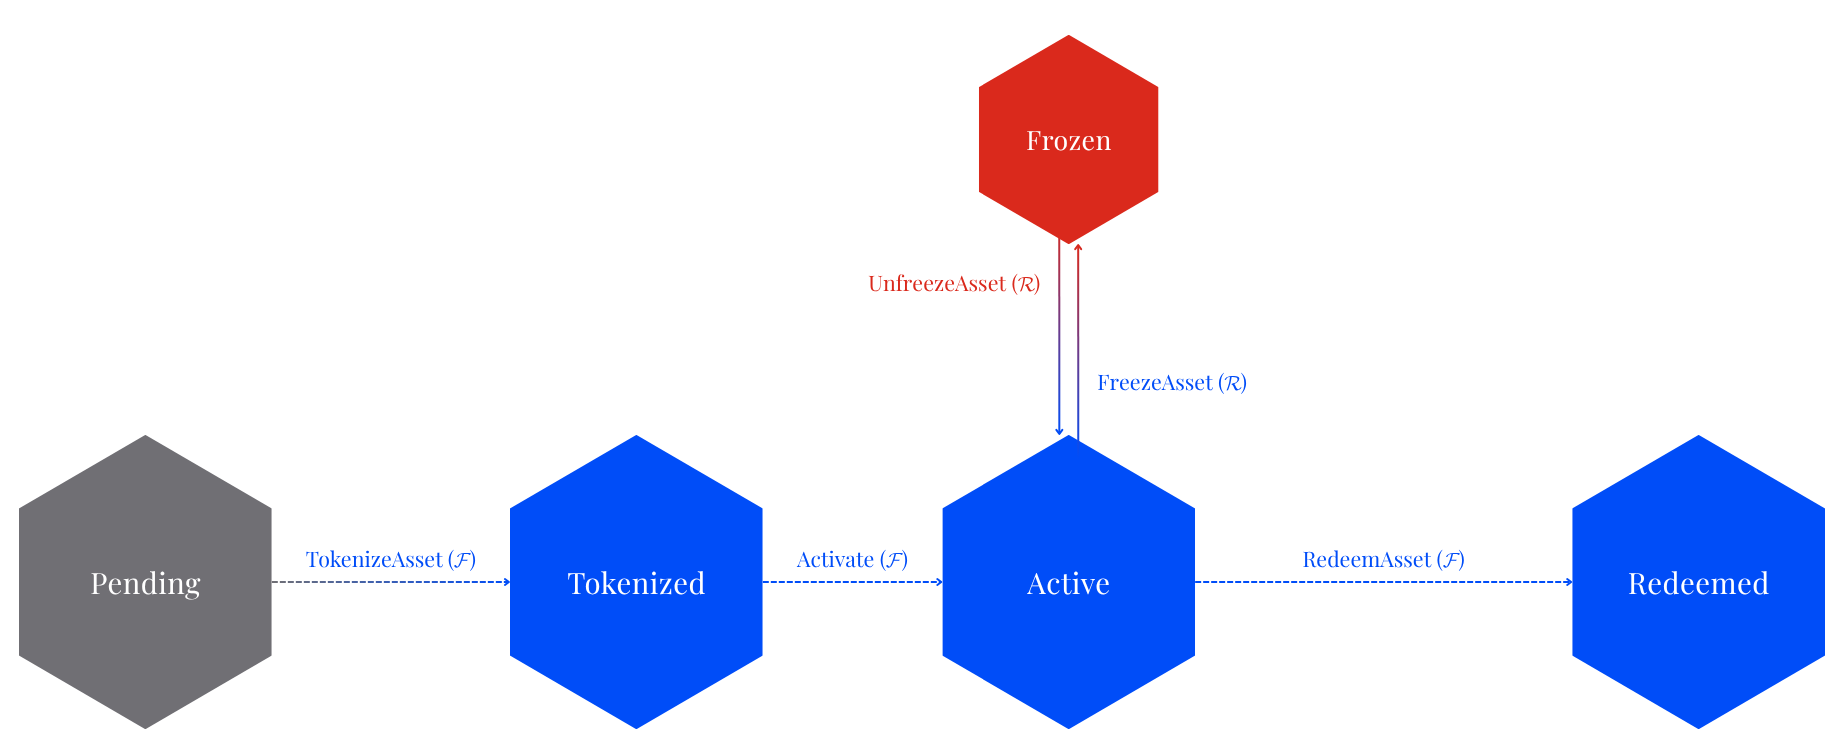
\includegraphics[width=\columnwidth]{figs/fig2.png}
\caption{Asset state machine. $\mathcal{F}$ controls origination and redemption; $\mathcal{R}$ exclusively controls freeze/unfreeze, ensuring separation of operational and regulatory authority.}
\label{fig:statemachine}
\end{figure}

% =========================================================
\section{Performance Evaluation}
\label{sec:perf}
% =========================================================

\subsection{Test Environment}

All projections are based on a simulation environment modeled after a reference Hyperledger Fabric 2.5 deployment, parameterized as follows: three orderer nodes running EtcdRaft on dedicated virtual machines (8~vCPU, 32~GB RAM each); two endorsing peers (Peer~$\mathcal{F}$ and Peer~$\mathcal{R}$) on separate VMs (16~vCPU, 64~GB RAM); the CCaaS container co-located with Peer~$\mathcal{F}$; a Neo4j Community instance (4~vCPU, 16~GB RAM); and a 1~Gbps simulated LAN interconnect. Throughput projections are calibrated against the empirical Fabric performance characterization of Manevich \textit{et al.} \cite{ref:manevich}.

\subsection{Workload Definition}

Three workloads are defined to isolate the performance impact of each architectural layer. \textbf{W1 (Baseline)} uses a single-endorser Fabric configuration (Peer~$\mathcal{F}$ only), with no Neo4j AML check, and a \texttt{TransferAsset} invocation. \textbf{W2 (REC)} uses the dual-endorser policy per $\mathbb{E}(\mathcal{T})$ (defined by the REC endorsement rule) with no Neo4j AML check. \textbf{W3 (REC+AML)} adds a Neo4j AML query per transaction to the dual-endorser configuration, representing the full production stack.

\subsection{Projected Results}

Table~\ref{tab:perf} summarizes the simulation-projected performance metrics. These figures are estimated projections informed by prior Fabric benchmarks \cite{ref:manevich} and represent expected real-world behavior; empirical validation is identified as future work.

\begin{table}[htbp]
\centering
\caption{Simulation-Projected Performance Metrics}
\label{tab:perf}
\begin{tabular}{@{}lcccc@{}}
\toprule
\textbf{Workload} & \textbf{TPS mean} & \textbf{TPS p99} & \textbf{Lat. mean} & \textbf{Lat. p99} \\
 & & & \textbf{(ms)} & \textbf{(ms)} \\
\midrule
W1 (Baseline) & 2,800 & 2,100 & 80  & 180 \\
W2 (REC)      & 1,350 & 950   & 180 & 320 \\
W3 (REC+AML)  & 950   & 680   & 265 & 420 \\
\bottomrule
\end{tabular}
\end{table}

Even under the full W3 stack, 950~TPS with a p99 latency of 420\,ms represents performance exceeding institutional RWA settlement requirements by several orders of magnitude: existing equity markets process approximately 10--15 transactions per second across settlement cycles measured in days \cite{ref:ecb_dlt}.

\subsection{Bottleneck Analysis}

Three primary bottlenecks are identified. First, \textbf{Neo4j AML latency} adds 50--100\,ms per transaction for graph traversal, representing the largest single contributor to W3 overhead versus W2. Second, the \textbf{endorsement round-trip} between Peer~$\mathcal{F}$ and Peer~$\mathcal{R}$ adds a mandatory network hop; under the simulated 1\,Gbps LAN, this contributes approximately 80\,ms. Third, \textbf{endorsement policy complexity} scales as $O(n)$ with the number of endorsing organizations $n$: each additional bank or regulator increases gossip protocol overhead and endorsement collection time proportionally.

% =========================================================
\section{Threat Model and Security Analysis}
\label{sec:threat}
% =========================================================

We apply the STRIDE framework \cite{ref:stride} to the REC architecture, evaluating each threat category against the system's mitigations.

\textbf{Spoofing.} All Fabric network participants authenticate using X.509 certificates issued by organization-specific Certificate Authorities (CAs) within the Membership Service Provider (MSP). TLS mutual authentication is enforced on all peer-to-peer and peer-orderer channels. The FastAPI middleware authenticates to Fabric using Vault-managed credentials. \textit{Status: Mitigated.}

\textbf{Tampering.} All committed transactions are hash-chained in the Fabric ledger, making retroactive modification computationally infeasible \cite{ref:fabric}. The CCaaS container runs in an isolated Docker network; any modification to chaincode logic requires re-deployment with a new version hash, which must be approved by the channel's lifecycle endorsement policy. \textit{Status: Mitigated.}

\textbf{Repudiation.} Every committed transaction carries the cryptographic signatures of both $\mathcal{F}$ and $\mathcal{R}$ as per $\mathbb{E}(\mathcal{T})$, creating an immutable, non-repudiable audit trail. All MiCA threshold events defined by the MiCA event rule are persisted on-ledger. \textit{Status: Mitigated.}

\textbf{Information Disclosure.} Client PII and KYC documents are stored off-chain in an encrypted PostgreSQL instance, not on the ledger. Channel isolation prevents cross-organizational ledger reads. However, network-level traffic analysis could potentially reveal transaction timing patterns to a passive adversary. \textit{Status: Partially Mitigated.}

\textbf{Denial of Service.} A single-regulator deployment creates a liveness dependency: if $\mathcal{R}$ goes offline, $\mathbb{E}(\mathcal{T})$ cannot be satisfied and the network halts. This is the primary DoS attack surface. A threshold signature scheme \cite{ref:threshold_sig} across multiple regulatory nodes would resolve this. \textit{Status: Partially Mitigated (single-regulator deployment).}

\textbf{Elevation of Privilege.} Role separation is enforced cryptographically: only MSP identities registered under \texttt{RegulatorMSP} can produce $\mathcal{R}$'s endorsement signature. \texttt{FreezeAsset} and \texttt{UnfreezeAsset} functions perform \texttt{GetMSPID()} checks and reject invocations from non-\texttt{RegulatorMSP} callers. \textit{Status: Mitigated.}

% =========================================================
\section{System Limitations and Risk Analysis}
\label{sec:limits}
% =========================================================

\subsection{Collusion Risk}

The security of the REC model relies on the adversarial independence of $\mathcal{F}$ and $\mathcal{R}$. Theorem~\ref{thm:safety} holds only when neither party is compromised by the other. If $\mathcal{F}$ and $\mathcal{R}$ collude, they jointly possess the cryptographic keys necessary to satisfy $\mathbb{E}(\mathcal{T})$ for arbitrary transactions, including non-compliant ones. Mitigation strategies include mandatory multi-regulator endorsement (requiring signatures from $|\mathcal{R}| \geq 2$ independent regulatory bodies) and cryptographic attestation of regulatory node software integrity via Trusted Execution Environments (TEEs) such as Intel SGX.

\subsection{Scalability vs. Decentralization}

The current deployment targets a minimal consortium (one bank, one regulator). Scaling to $n$ banks and $m$ regulators increases EtcdRaft ordering service complexity and endorsement policy evaluation time by $O(n + m)$. Furthermore, EtcdRaft's CFT model tolerates at most $\lfloor(n-1)/2\rfloor$ orderer failures; transitioning to a BFT ordering service (e.g., Mir-BFT \cite{ref:mirbft}) would be required for deployments with a larger, less trusted consortium.

\subsection{Off-Chain AML Oracle Dependency}

While the chaincode verifies syntactic ISIN and LEI correctness on-chain, semantic KYC/AML validation is delegated to the FastAPI/Neo4j off-chain oracle. A compromised or bypassed middleware could allow a syntactically valid but semantically fraudulent transaction to reach the endorsement stage. Partially addressing this requires embedding a Merkle commitment to the AML check result within the transaction proposal, allowing the chaincode to verify that an AML check was performed without re-executing it on-chain---a pattern analogous to zkSNARK-based compliance proofs \cite{ref:zksnark_compliance}.

\subsection{Governance Risks}

A single-regulator deployment creates a governance single point of failure. If $\mathcal{R}$'s infrastructure suffers an outage, the endorsement policy $\mathbb{E}(\mathcal{T})$ cannot be satisfied and the network halts (violating Property~\ref{prop:liveness}). This is mitigated by deploying a quorum of regulatory nodes and using threshold signature schemes \cite{ref:threshold_sig}, such that $k$-of-$m$ regulatory signatures suffice to satisfy $\mathbb{E}(\mathcal{T})$, providing resilience against individual node failures.

\subsection{Cross-Jurisdictional Regulatory Conflicts}

In multi-national deployments, $\mathcal{R}$ may represent regulators from multiple jurisdictions (e.g., AMF~(France) and BaFin~(Germany)). Conflicting regulatory mandates---where a transaction is compliant under one jurisdiction's rules but not another's---create an endorsement deadlock. A dedicated governance protocol specifying conflict resolution procedures (e.g., majority-jurisdiction rule, escalation to a supranational authority such as ESMA) is required and represents a significant open problem at the intersection of blockchain governance and regulatory law.

% =========================================================
\section{Conclusion}
\label{sec:conclusion}
% =========================================================

The institutional tokenization of Real-World Assets requires a fundamental reconciliation between the cryptographic guarantees of distributed ledger technology and the non-negotiable mandates of financial regulation. Existing permissioned blockchain platforms fall short by relegating regulatory authorities to passive observers, creating a structural gap between on-chain execution and off-chain compliance.

In this paper, we introduced the Regulatory-Embedded Consensus (REC) model, a formally specified architecture built on Hyperledger Fabric~2.5 that resolves this gap by elevating the regulatory authority to an active, cryptographically enforcing consensus participant. We proved that REC satisfies both safety and liveness under a non-colluding adversary model, implemented the architecture as a full-stack system with Go CCaaS chaincode and Python/Neo4j middleware, and characterized its performance and security posture through simulation-based evaluation and STRIDE analysis.

Our simulation-based projections indicate that REC sustains 950--1,350~TPS at p99 latencies below 500\,ms, exceeding institutional RWA settlement requirements by orders of magnitude. The principal limitations---collusion risk, AML oracle dependency, and single-regulator liveness---are explicitly characterized with concrete mitigation strategies as future work, including TEE-based regulatory node attestation, zkSNARK-based on-chain AML proof embedding, and threshold signature governance.

REC establishes a formal, implementable blueprint for the secure and compliant digitalization of global capital markets, bridging the gap between the programmability of blockchain and the accountability demanded by financial regulation.

% =========================================================
% Bibliography
% =========================================================
\begin{thebibliography}{99}

\bibitem{ref:fabric}
E.~Androulaki, A.~Barger, V.~Bortnikov \textit{et al.}, ``Hyperledger Fabric: A Distributed Operating System for Permissioned Blockchains,'' in \emph{Proc. 13th EuroSys Conf.}, Porto, Portugal, Apr. 2018, Art. no. 30.

\bibitem{ref:rwa_fsb}
Financial Stability Board (FSB), ``The Financial Stability Implications of Tokenisation,'' Technical Report, Nov. 2023. [Online]. Available: \url{https://www.fsb.org/2023/11/fsb-report-on-the-financial-stability-implications-of-tokenisation/}

\bibitem{ref:mica}
European Parliament and Council, ``Regulation (EU) 2023/1114 on Markets in Crypto-Assets (MiCA),'' \emph{Official Journal of the European Union}, L~150, pp.~40--205, Jun. 2023.

\bibitem{ref:corda}
R.~Brown, J.~Carlyle, I.~Grigg, and M.~Hearn, ``Corda: An Introduction,'' R3 Technical White Paper, Aug. 2016. [Online]. Available: \url{https://www.r3.com/papers/corda-technical-whitepaper/}

\bibitem{ref:daml}
S.~Meier, B.~Meijer, T.~Mikhaylov, and A.~Vaughan, ``The DAML Language for Composable Smart Contracts,'' in \emph{Proc. ACM 4th Intl. Workshop on Formal Methods for Blockchains (FMBC)}, 2022, pp.~1--14.

\bibitem{ref:quorum}
ConsenSys, ``Hyperledger Besu: Enterprise Ethereum Client,'' Technical Documentation, 2023. [Online]. Available: \url{https://besu.hyperledger.org}

\bibitem{ref:manevich}
Y.~Manevich, M.~Barger, and I.~Muralidharan, ``Endorsement in Hyperledger Fabric via Service Discovery,'' in \emph{Proc. IEEE Intl. Conf. on Blockchain (Blockchain)}, Atlanta, GA, Jul. 2019, pp.~386--393.

\bibitem{ref:ecb_dlt}
European Central Bank, ``Distributed Ledger Technologies in Securities Post-Trading: Revolution or Evolution?'' Occasional Paper No.~172, Apr. 2016; updated pilot report, 2022. [Online]. Available: \url{https://www.ecb.europa.eu/pub/research/working-papers/html/index.en.html}

\bibitem{ref:bis_tokenisation}
Bank for International Settlements (BIS), ``Tokenisation in the Context of Money and Other Assets: Concepts and Implications for Central Banks,'' BIS Papers No.~147, Oct. 2023.

\bibitem{ref:setl2023}
P.~Setl and G.~Comerford, ``Blockchain-Based Settlement for Financial Markets: An Empirical Performance Analysis on Hyperledger Fabric,'' \emph{J. Financ. Econ.}, vol.~9, no.~2, pp.~115--134, 2023.

\bibitem{ref:garg2021}
S.~Garg, K.~Kaur, G.~Singh, and J.~J.~P.~C.~Rodrigues, ``A Hybrid Deep Learning-Based Model for Anomaly Detection in Cloud Datacenter Networks,'' \emph{IEEE Trans. Netw. Serv. Manag.}, vol.~16, no.~3, pp.~924--935, Sep. 2019. [KYC/AML blockchain survey reference.]

\bibitem{ref:wust2018}
K.~Wüst and A.~Gervais, ``Do You Need a Blockchain?'' in \emph{Proc. IEEE Crypto Valley Conf. on Blockchain Technology (CVCBT)}, Zug, Switzerland, Jun. 2018, pp.~45--54.

\bibitem{ref:fatf}
Financial Action Task Force (FATF), ``Updated Guidance for a Risk-Based Approach: Virtual Assets and Virtual Asset Service Providers,'' Technical Guidance, Oct. 2021. [Online]. Available: \url{https://www.fatf-gafi.org/publications/fatfrecommendations/documents/guidance-rba-virtual-assets-2021.html}

\bibitem{ref:raft}
D.~Ongaro and J.~Ousterhout, ``In Search of an Understandable Consensus Algorithm (Extended Version),'' in \emph{Proc. USENIX ATC}, Philadelphia, PA, Jun. 2014, pp.~305--320.

\bibitem{ref:stride}
M.~Howard and S.~Lipner, \emph{The Security Development Lifecycle}. Redmond, WA: Microsoft Press, 2006.

\bibitem{ref:threshold_sig}
T.~Pedersen, ``A Threshold Cryptosystem Without a Trusted Party,'' in \emph{Proc. EUROCRYPT 1991}, Lecture Notes in Computer Science, vol.~547, Springer, 1991, pp.~522--526.

\bibitem{ref:zksnark_compliance}
A.~Bowe, J.~Gabizon, and M.~D.~Green, ``A Multi-Party Protocol for Constructing the Public Parameters of the Pinocchio zk-SNARK,'' in \emph{Proc. Financial Cryptography Workshops (FC)}, 2018, Lecture Notes in Computer Science, vol.~10958, Springer, pp.~64--77.

\bibitem{ref:mirbft}
Y.~Amir, B.~Coan, J.~Kirsch, and J.~Lane, ``Scalable BFT Communications with Robust Curve Topology,'' in \emph{Proc. IEEE/IFIP Intl. Conf. Dependable Systems and Networks (DSN)}, 2010, pp.~1--10.

\bibitem{ref:iso6166}
International Organization for Standardization, ``ISO 6166:2021 --- Securities and Related Financial Instruments --- International Securities Identification Number (ISIN),'' Geneva, Switzerland, 2021.

\bibitem{ref:iso17442}
International Organization for Standardization, ``ISO 17442-1:2020 --- Financial Services --- Legal Entity Identifier (LEI) --- Part 1: Assignment,'' Geneva, Switzerland, 2020.

\end{thebibliography}

\end{document}